\begin{figure*}[t!]
\centering
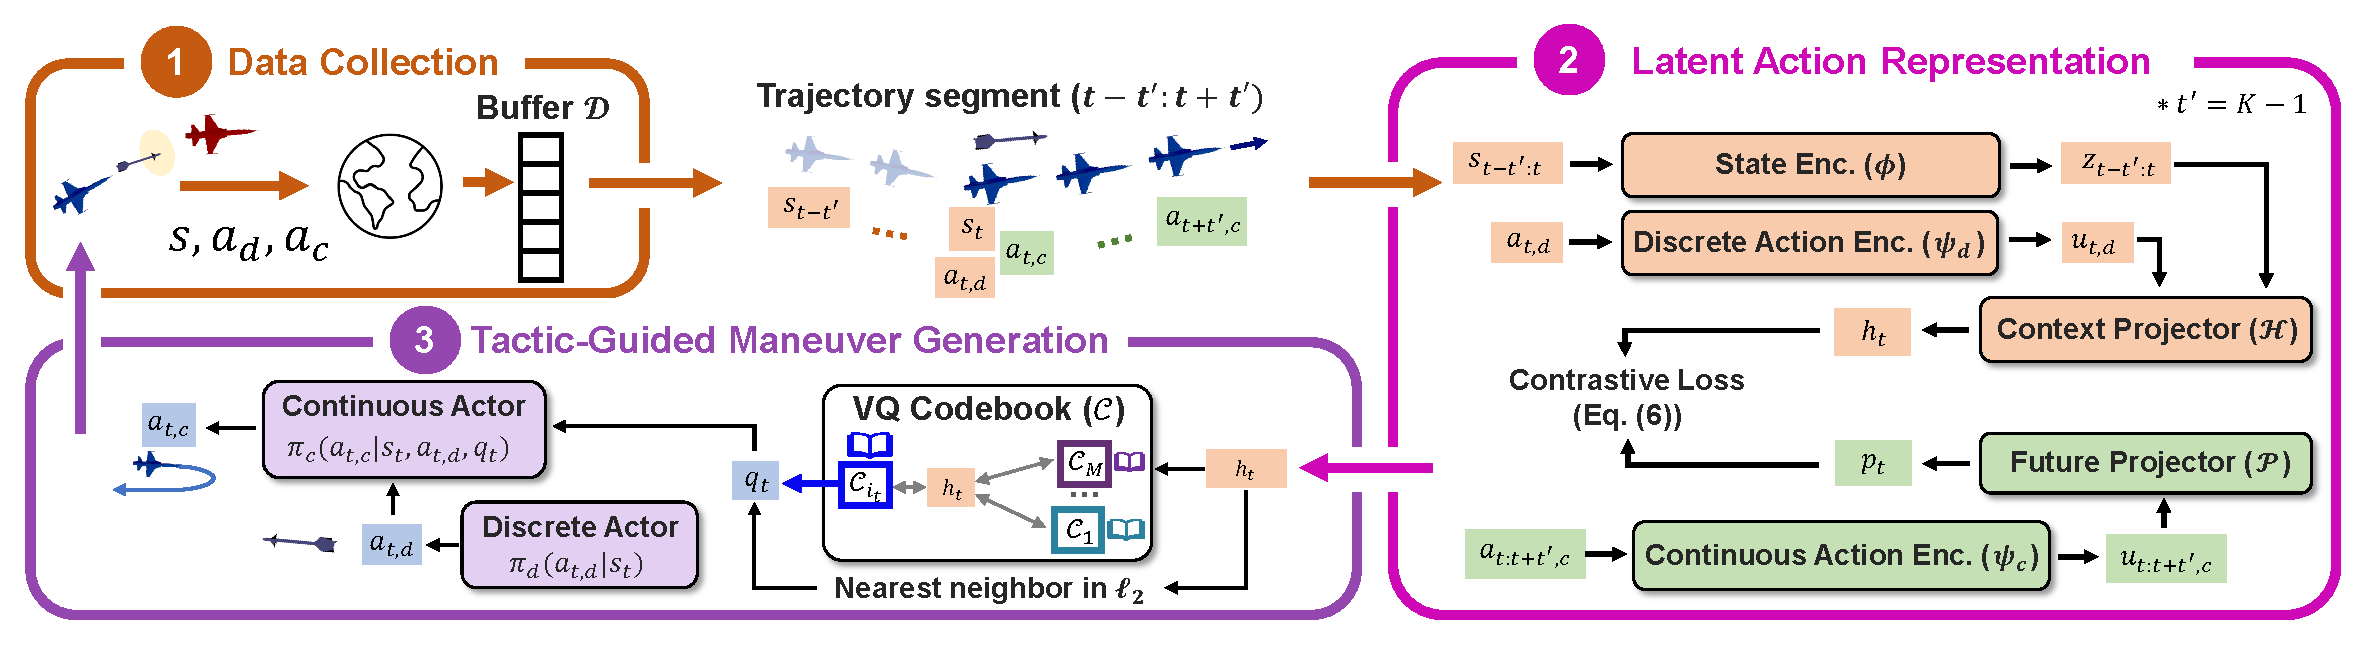
\includegraphics[width=1\textwidth]{Figures/fig_2.pdf}
\caption{Overview of TART: (1) The agent interacts with the environment and collects a set of trajectories. (2) A mutual information objective guides the clustering of given trajectories into multiple tactical modes through contrastive learning (Sec. III-B). (3) The resulting distinct modes are then mapped to discrete vectors via vector quantization (VQ). The continuous actor distinguishes between the modes and generates multi-modal maneuver distributions accordingly (Sec. III-C).
}
\vspace{-10pt}
\label{fig:TART}
\end{figure*}

In this paper, we build on a Parameterized Action Markov Decision Process (PAMDP) $\langle\mathcal{S}, \mathcal{X}, P, \gamma, \mathcal{R}\rangle$, defined with a state space $\mathcal{S}$, parameterized action space $\mathcal{X}$, transition function $P : \mathcal{S} \times \mathcal{X} \times \mathcal{S} \rightarrow \mathbb{R}$, discount factor $\gamma \in [0, 1)$, and reward function~$\mathcal{R} : \mathcal{S} \times \mathcal{X} \rightarrow \mathbb{R}$~\cite{masson2016reinforcement}.
Specifically, we extend the standard PAMDP framework to incorporate a discrete-continuous hybrid action space defined as Cartesian product $\mathcal{X}=\mathcal{A}_d \times \mathcal{A}_c$, where $\mathcal{A}_d = \{ a_{d,1}, ..., a_{d, m}\}$ is a finite set of $m$ discrete resource decisions and $\mathcal{A}_c \subseteq\mathbb{R}^n$ is the $n$-dimensional continuous control space.
A hybrid action is denoted $a=(a_d, a_c)$.
The agent maximizes the expected discounted return $J(\pi)=\mathbb{E}_\pi[\sum_{t=0}^\infty\gamma^t\mathcal{R}(s_t, a_t)]$, where the policy factorizes as $\pi(a_d, a_c|s)=\pi_d(a_d|s)\pi_c(a_c|s, a_d)$.
We recall the value functions, $V^\pi(s):=\mathbb{E}_\pi[\sum_{t\geq0}\gamma^t\mathcal{R}(s_t, a_t) | s_0=s]$ and $Q^\pi(s, a):=\mathcal{R}(s,a) + \gamma\mathbb{E}_{s'\sim P(\cdot|s,a)}[V^\pi(s')]$.
The optimal value functions are denoted as $V^*(s)=\sup_\pi V^\pi(s)$ and $Q^*(s,a)=\sup_\pi Q^\pi(s,a)$.